\documentclass[12pt, a4paper]{article}
\usepackage[utf8]{inputenc}
\usepackage[english]{babel}
\usepackage{amsmath}
\usepackage{csquotes}
\usepackage{mathtools}
\usepackage{graphicx}
\usepackage{geometry}
\usepackage{setspace}
\usepackage{longtable}
\usepackage[colorlinks=true, allcolors=blue]{hyperref}

\usepackage[style=authoryear]{biblatex}
\addbibresource{Bibliography.bib}

\geometry{top = 2.5cm, bottom = 2.5cm, left= 3cm, right= 3cm}

\title{Forbes' bar}
\author{Lee Farrugia \\ Experiment 9 \\ Group 1A}

\date{$25^{\text{th}}$ October 2021}

\begin{document}

\maketitle

\section*{Aim}
The aim of this experiment was to use the thermal conductivity of copper in heat loss calculations in order to determine the specific heat capacity of the copper provided.

\section*{Diagram}
\begin{figure}[ht]
    \centering
    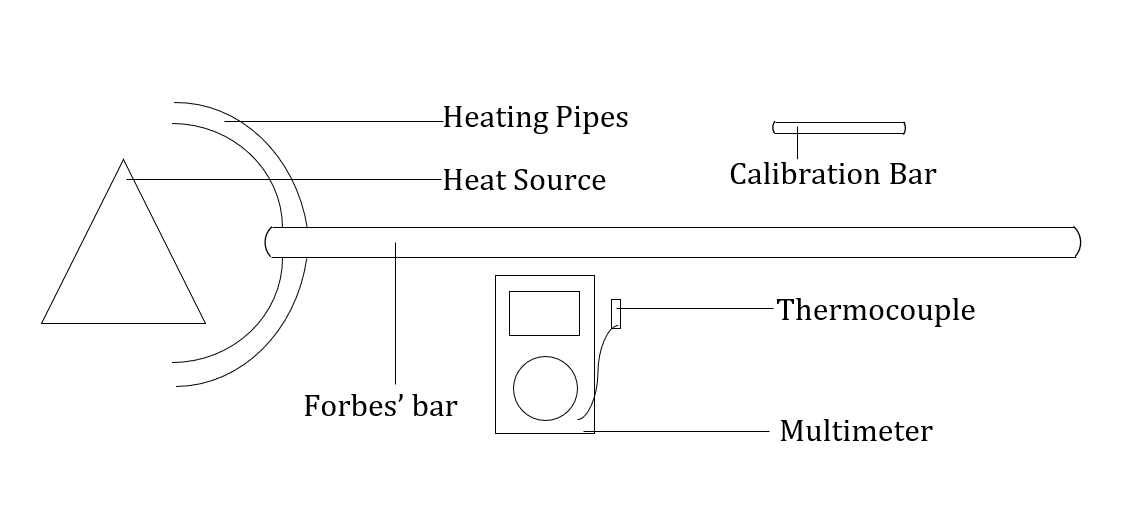
\includegraphics[width=\textwidth]{Experiment 9 Diagram.png}
    \caption{Forbes' bar Diagram}
    \label{fig:Apparatus diagram}
\end{figure}

\section*{List of Apparatus}

Copper bar with large holes (Forbes' bar), copper bar with hole in center (calibration bar), boiler, hot plate, multi-meter with thermocouple, vernier, electronic balance, meter ruler

\section*{Procedure}
\begin{enumerate}
    \item The boiler was filled with water and the heater was switched on. Since the heating of the Forbes' bar took more than two hours this was done before.
    \item The thermocouple was connected to the multi-meter and set to read the temperature.
    \item The temperature was read at various positions by inserting the thermocouple inside the holes of the Forbes' bar.
    \item This was repeated multiple times until the temperature of the Forbes' bar did not vary.
    \item The temperature $\theta$ was measured and recorded in Table \ref{tab: Table 1} at each position $x$ along the Forbes' bar. This was done until four data sets were obtained. In addition the distance $x$ was measured from the middle of the hot water supply tubes, and the distance between each hole was assumed to be 1cm.
    \item The boiler was switched off so that the Forbes' bar cooled down.
    \item The length, diameter of the Forbes' bar was recorded in Table \ref{tab:Table 2}.
    \item The length, diameter and mass of the calibration were measured and recorded in Table \ref{tab:Table 4}.
    \item The thermocouple was placed deep into the calibration bar.
    \item The calibration bar was heated using the hot plate to 120 $^{\circ}$C.
    \item The heated thermocouple was moved quickly to the sponge provided. 
    \item The variation in temperature $\phi$ of the calibration bar was measured every 15s and recorded in Table \ref{tab:Table 3}.
\end{enumerate}

\section*{Precautions}
\begin{itemize}
    \item[-] The heated parts were not touched until they were cool.
    \item[-] It was made sure that no water was spilled over the electronic parts.
    \item[-] The electric components were not touched with wet hands.
    \item[-] The mass of the calibration bar was taken by first putting it on the electronic balance and then removing it and replacing it on top of the electronic balance.
    \item[-] The temperature reading of the Forbes' bar was taken in alternate sequence.
    \item[-] When taking the diameter readings the vernier caliper was locked.
    \item[-] When taking the diameters, lengths with the vernier calipers, they were taken perpendicularly to each other.
\end{itemize}

\section*{Sources of Error}
\begin{enumerate}
    \item[-] The Forbes' bar was not made uniformly of the same material.
    \item[-] The holes along the surface of the Forbes' bar may have not been directly in the middle.
    \item[-] The holes along the surface of the Forbes' bar may have not have the same diameter and/or depth.
    \item[-] The thermocouple may have been at the same height in the hole when taking readings in the Forbes' bar. 
    \item[-] the thermocouple may not have been at the same spot when taking the different reading for the calibration bar.
    \item[-] Air currents caused by the open windows and moving students may have caused fluctuations in the readings obtained from the thermocouple.
\end{enumerate}

\section*{Data and Graphs}

\begin{center}
\begin{longtable}{| c | c | c | c | c | c | c | c |}
    \caption{Forbes' bar Temperature Readings} \label{tab: Table 1}\\
    \hline \textbf{$x_1 {\textmd{/m}}$} & \textbf{$F_1 {\textmd{/} ^{\circ} \textmd{C}}$} & \textbf{$x_2 {\textmd{/m}}$} & \textbf{$F_2 {\textmd{/} ^{\circ} \textmd{C}}$} & \textbf{$x_3 {\textmd{/m}}$} & \textbf{$F_3 {\textmd{/} ^{\circ} \textmd{C}}$} & \textbf{$x_4 {\textmd{/m}}$} & \textbf{$F_4 {\textmd{/} ^{\circ} \textmd{C}}$} \\ \hline 
    
    \hline \text{\textpm\ 0.01} & \text{\textpm\ 1} & \text{\textpm\ 0.01} & \text{\textpm\ 1} & \text{\textpm\ 0.01} & \text{\textpm\ 1} & \text{\textpm\ 0.01} & \text{\textpm\ 1} \\ \hline 
    \endfirsthead
    
    \hline \textbf{$x_1 {\textmd{/m}}$} & \textbf{$F_1 {\textmd{/} ^{\circ} \textmd{C}}$} & \textbf{$x_2 {\textmd{/m}}$} & \textbf{$F_2 {\textmd{/} ^{\circ} \textmd{C}}$} & \textbf{$x_3 {\textmd{/m}}$} & \textbf{$F_3 {\textmd{/} ^{\circ} \textmd{C}}$} & \textbf{$x_4 {\textmd{/m}}$} & \textbf{$F_4 {\textmd{/} ^{\circ} \textmd{C}}$} \\ \hline 

    \hline \text{\textpm\ 0.01} & \text{\textpm\ 1} & \text{\textpm\ 0.01} & \text{\textpm\ 1} & \text{\textpm\ 0.01} & \text{\textpm\ 1} & \text{\textpm\ 0.01} & \text{\textpm\ 1} \\ \hline 
    \endhead

    \hline
    \endfoot

0.081 & 90 & 0.081 & 90 & 0.081 & 90 & 0.081 & 90 \\
0.091 & 88 & 0.091 & 88 & 0.091 & 88 & 0.091 & 88 \\
0.101 & 86 & 0.101 & 86 & 0.101 & 86 & 0.101 & 85 \\
0.111 & 84 & 0.111 & 84 & 0.111 & 84 & 0.111 & 82 \\
0.121 & 82 & 0.121 & 82 & 0.121 & 81 & 0.121 & 80 \\
0.131 & 79 & 0.131 & 79 & 0.131 & 79 & 0.131 & 79 \\
0.141 & 77 & 0.141 & 77 & 0.141 & 78 & 0.141 & 77 \\
0.151 & 75 & 0.151 & 75 & 0.151 & 77 & 0.151 & 76 \\
0.161 & 73 & 0.161 & 73 & 0.161 & 75 & 0.161 & 75 \\
0.171 & 71 & 0.171 & 71 & 0.171 & 73 & 0.171 & 72 \\
0.181 & 69 & 0.181 & 69 & 0.181 & 71 & 0.181 & 70 \\
0.191 & 68 & 0.191 & 68 & 0.191 & 70 & 0.191 & 69 \\
0.201 & 67 & 0.201 & 67 & 0.201 & 68 & 0.201 & 68 \\
0.211 & 65 & 0.211 & 65 & 0.211 & 66 & 0.211 & 66 \\
0.221 & 64 & 0.221 & 63 & 0.221 & 65 & 0.221 & 64 \\
0.231 & 62 & 0.231 & 62 & 0.231 & 63 & 0.231 & 63 \\
0.241 & 61 & 0.241 & 60 & 0.241 & 62 & 0.241 & 62 \\
0.251 & 59 & 0.251 & 59 & 0.251 & 61 & 0.251 & 60 \\
0.261 & 58 & 0.261 & 58 & 0.261 & 59 & 0.261 & 59 \\
0.271 & 57 & 0.271 & 57 & 0.271 & 58 & 0.271 & 58 \\
0.281 & 56 & 0.281 & 56 & 0.281 & 57 & 0.281 & 57 \\
0.291 & 55 & 0.291 & 55 & 0.291 & 56 & 0.291 & 56 \\
0.301 & 54 & 0.301 & 53 & 0.301 & 54 & 0.301 & 54 \\
0.311 & 53 & 0.311 & 52 & 0.311 & 54 & 0.311 & 53 \\
0.321 & 52 & 0.321 & 51 & 0.321 & 53 & 0.321 & 52 \\
0.331 & 51 & 0.331 & 51 & 0.331 & 52 & 0.331 & 51 \\
0.341 & 50 & 0.341 & 50 & 0.341 & 51 & 0.341 & 50 \\
0.351 & 49 & 0.351 & 49 & 0.351 & 49 & 0.351 & 49 \\
0.361 & 48 & 0.361 & 48 & 0.361 & 48 & 0.361 & 48 \\
0.371 & 47 & 0.371 & 47 & 0.371 & 47 & 0.371 & 47 \\
0.381 & 47 & 0.381 & 46 & 0.381 & 47 & 0.381 & 47 \\
0.391 & 46 & 0.391 & 46 & 0.391 & 46 & 0.391 & 46 \\
0.401 & 45 & 0.401 & 45 & 0.401 & 45 & 0.401 & 45 \\
0.411 & 45 & 0.411 & 45 & 0.411 & 44 & 0.411 & 44 \\
0.421 & 44 & 0.421 & 44 & 0.421 & 44 & 0.421 & 44 \\
0.431 & 44 & 0.431 & 44 & 0.431 & 43 & 0.431 & 44 \\
0.441 & 43 & 0.441 & 43 & 0.441 & 43 & 0.441 & 43 \\
0.451 & 43 & 0.451 & 43 & 0.451 & 42 & 0.451 & 42 \\
0.461 & 42 & 0.461 & 42 & 0.461 & 42 & 0.461 & 42 \\
0.471 & 42 & 0.471 & 42 & 0.471 & 41 & 0.471 & 42 \\
0.481 & 41 & 0.481 & 41 & 0.481 & 41 & 0.481 & 41 \\
0.491 & 41 & 0.491 & 41 & 0.491 & 41 & 0.491 & 41 \\
0.501 & 41 & 0.501 & 41 & 0.501 & 40 & 0.501 & 41 \\
0.511 & 41 & 0.511 & 40 & 0.511 & 40 & 0.511 & 40 \\
0.521 & 40 & 0.521 & 40 & 0.521 & 40 & 0.521 & 40 \\
0.521 & 40 & 0.521 & 40 & 0.521 & 40 & 0.521 & 40 \\
0.531 & 40 & 0.531 & 40 & 0.531 & 39 & 0.531 & 39 \\
0.541 & 39 & 0.541 & 39 & 0.541 & 39 & 0.541 & 39 \\
0.551 & 39 & 0.551 & 39 & 0.551 & 39 & 0.551 & 39 \\
0.561 & 39 & 0.561 & 39 & 0.561 & 39 & 0.561 & 39 \\
0.571 & 39 & 0.571 & 38 & 0.571 & 39 & 0.571 & 38 \\
0.581 & 39 & 0.581 & 38 & 0.581 & 39 & 0.581 & 38 \\
0.591 & 39 & 0.591 & 38 & 0.591 & 38 & 0.591 & 38 \\
0.601 & 39 & 0.601 & 38 & 0.601 & 38 & 0.601 & 38 \\
0.611 & 39 & 0.611 & 38 & 0.611 & 38 & 0.611 & 38 \\
0.621 & 38 & 0.621 & 38 & 0.621 & 38 & 0.621 & 38 \\
0.631 & 38 & 0.631 & 38 & 0.631 & 38 & 0.631 & 38 \\
0.641 & 38 & 0.641 & 38 & 0.641 & 38 & 0.641 & 38 \\
0.651 & 38 & 0.651 & 38 & 0.651 & 38 & 0.651 & 38

\end{longtable}
\end{center}

\begin{center}
\begin{longtable}{| c | c | c | c |}
    \caption{Forbes' bar Length and Diameters} \label{tab:Table 2}\\
    \hline \textbf{$F_l {\textmd{/m}}$} & \textbf{$F_{d1} {\textmd{/m}}$} & \textbf{$F_{d2} {\textmd{/m}}$} & \textbf{$F_{d3} {\textmd{/m}}$} \\ \hline 
    
    \hline \text{\textpm\ 0.01} & \text{\textpm\ 5$\times 10^{-5}$} & \text{\textpm\  5$\times 10^{-5}$} & \text{\textpm\  5$\times 10^{-5}$} \\ \hline 
    \endfirsthead
    
    \hline \textbf{$F_l {\textmd{/m}}$} & \textbf{$F_{d1} {\textmd{/m}}$} & \textbf{$F_{d2} {\textmd{/m}}$} & \textbf{$F_{d3} {\textmd{/m}}$} \\ \hline 

    \hline \text{\textpm\ 0.01} & \text{\textpm\ 5$\times 10^{-5}$} & \text{\textpm\  5$\times 10^{-5}$} & \text{\textpm\  5$\times 10^{-5}$} \\ \hline 
    \endhead

    \hline
    \endfoot

0.660 & 0.03200 & 0.03195 & 0.03170 \\
0.659 & 0.03200 & 0.03195 & 0.03180 \\
0.659 &         &         &         \\

\end{longtable}
\end{center}

\begin{center}
\begin{longtable}{| c | c | c | c | c | c |}
    \caption{Calibration bar Temperature Readings} \label{tab:Table 3}\\
    \hline \textbf{$t_1 {\textmd{/s}}$} & \textbf{$C_1 {\textmd{/} ^{\circ} \textmd{C}}$} & \textbf{$t_2 {\textmd{/s}}$} & \textbf{$C_2 {\textmd{/} ^{\circ} \textmd{C}}$} & \textbf{$t_3 {\textmd{/s}}$} & \textbf{$C_3 {\textmd{/} ^{\circ} \textmd{C}}$} \\ \hline 
    
    \hline \text{\textpm\ 0.01} & \text{\textpm\ 1} & \text{\textpm\ 0.01} & \text{\textpm\ 1} & \text{\textpm\ 0.01} & \text{\textpm\ 1} \\ \hline 
    \endfirsthead
    
    \hline \textbf{$t_1 {\textmd{/s}}$} & \textbf{$C_1 {\textmd{/} ^{\circ} \textmd{C}}$} & \textbf{$t_2 {\textmd{/s}}$} & \textbf{$C_2 {\textmd{/} ^{\circ} \textmd{C}}$} & \textbf{$t_3 {\textmd{/s}}$} & \textbf{$C_3 {\textmd{/} ^{\circ} \textmd{C}}$} \\ \hline 

    \hline \text{\textpm\ 0.01} & \text{\textpm\ 1} & \text{\textpm\ 0.01} & \text{\textpm\ 1} & \text{\textpm\ 0.01} & \text{\textpm\ 1} \\ \hline 
    \endhead

    \hline
    \endfoot
    
0.0   & 120 & 0.0   & 120 & 0.0   & 120 \\
15.0  & 118 & 15.0  & 117 & 15.0  & 118 \\
30.0  & 115 & 30.0  & 115 & 30.0  & 115 \\
45.0  & 113 & 45.0  & 112 & 45.0  & 113 \\
60.0  & 110 & 60.0  & 110 & 60.0  & 110 \\
75.0  & 108 & 75.0  & 108 & 75.0  & 108 \\
90.0  & 106 & 90.0  & 106 & 90.0  & 106 \\
105.0 & 104 & 105.0 & 104 & 105.0 & 104 \\
120.0 & 102 & 120.0 & 102 & 120.0 & 102 \\
135.0 & 100 & 135.0 & 100 & 135.0 & 100 \\
150.0 & 98  & 150.0 & 98  & 150.0 & 99  \\
165.0 & 96  & 165.0 & 96  & 165.0 & 97  \\
180.0 & 94  & 180.0 & 94  & 180.0 & 95  \\
195.0 & 93  & 195.0 & 92  & 195.0 & 94  \\
210.0 & 91  & 210.0 & 91  & 210.0 & 92  \\
225.0 & 89  & 225.0 & 89  & 225.0 & 90  \\
240.0 & 88  & 240.0 & 88  & 240.0 & 89  \\
255.0 & 86  & 255.0 & 86  & 255.0 & 88  \\
270.0 & 85  & 270.0 & 84  & 270.0 & 86  \\
285.0 & 83  & 285.0 & 83  & 285.0 & 85  \\
300.0 & 82  & 300.0 & 82  & 300.0 & 84  \\
315.0 & 80  & 315.0 & 80  & 315.0 & 82  \\
330.0 & 79  & 330.0 & 79  & 330.0 & 81  \\
345.0 & 78  & 345.0 & 78  & 345.0 & 80  \\
360.0 & 77  & 360.0 & 76  & 360.0 & 79  \\
375.0 & 76  & 375.0 & 75  & 375.0 & 78  \\
390.0 & 74  & 390.0 & 74  & 390.0 & 77  \\
405.0 & 73  & 405.0 & 73  & 405.0 & 75  \\
420.0 & 72  & 420.0 & 72  & 420.0 & 74  \\
435.0 & 71  & 435.0 & 71  & 435.0 & 73  \\
450.0 & 70  & 450.0 & 70  & 450.0 & 72  \\
465.0 & 69  & 465.0 & 69  & 465.0 & 71  \\
480.0 & 68  & 480.0 & 68  & 480.0 & 70  \\
495.0 & 67  & 495.0 & 67  & 495.0 & 69  \\
510.0 & 66  & 510.0 & 66  & 510.0 & 68  \\
525.0 & 65  & 525.0 & 65  & 525.0 & 67  \\
540.0 & 64  & 540.0 & 64  & 540.0 & 67  \\
555.0 & 63  & 555.0 & 63  & 555.0 & 66  \\
570.0 & 62  & 570.0 & 62  & 570.0 & 65  \\
585.0 & 61  & 585.0 & 62  & 585.0 & 64  \\
600.0 & 60  & 600.0 & 61  & 600.0 & 63  \\
615.0 & 60  & 615.0 & 60  & 615.0 & 62  \\
630.0 & 59  & 630.0 & 59  & 630.0 & 61  \\
645.0 & 58  & 645.0 & 59  & 645.0 & 61  \\
660.0 & 57  & 660.0 & 58  & 660.0 & 60  \\
675.0 & 57  & 675.0 & 57  & 675.0 & 59  \\
690.0 & 56  & 690.0 & 57  & 690.0 & 57  \\
705.0 & 56  & 705.0 & 56  & 705.0 & 56  \\
720.0 & 55  & 720.0 & 55  & 720.0 & 55  \\
735.0 & 54  & 735.0 & 55  & 735.0 & 55  \\
750.0 & 54  & 750.0 & 54  & 750.0 & 54  \\
765.0 & 53  & 765.0 & 54  & 765.0 & 53  \\
780.0 & 53  & 780.0 & 53  & 780.0 & 53  \\
795.0 & 52  & 795.0 & 52  & 795.0 & 52  \\
810.0 & 52  & 810.0 & 52  & 810.0 & 52  \\
825.0 & 51  & 825.0 & 51  & 825.0 & 51  \\
840.0 & 50  & 840.0 & 50  & 840.0 & 50  \\
\end{longtable}
\end{center}

\begin{center}
\begin{longtable}{| c | c | c | c | c |}
    \caption{Calibration bar Length, Diameter, Mass Readings} \label{tab:Table 4}\\
    \hline \textbf{$C_m {\textmd{/kg}}$} & \textbf{$C_{d1} {\textmd{/m}}$} & \textbf{$C_{d2} {\textmd{/m}}$} & \textbf{$C_{d3} {\textmd{/m}}$} & \textbf{$C_l {\textmd{/m}}$} \\ \hline 
    
    \hline \textbf{\textpm\ 0.0001} & \textbf{\textpm\  5$\times 10^{-5}$} & \textbf{\textpm\  5$\times 10^{-5}$} & \textbf{\textpm\  5$\times 10^{-5}$} & \textbf{\textpm\  5$\times 10^{-5}$} \\ \hline 
    \endfirsthead
    
    \hline \textbf{$C_m {\textmd{/kg}}$} & \textbf{$C_{d1} {\textmd{/m}}$} & \textbf{$C_{d2} {\textmd{/m}}$} & \textbf{$C_{d3} {\textmd{/m}}$} & \textbf{$C_l {\textmd{/m}}$} \\ \hline 

    \hline \textbf{\textpm\ 0.0001} & \textbf{\textpm\  5$\times 10^{-5}$} & \textbf{\textpm\  5$\times 10^{-5}$} & \textbf{\textpm\  5$\times 10^{-5}$} & \textbf{\textpm\  5$\times 10^{-5}$} \\ \hline 
    \endhead

    \hline
    \endfoot
0.0422 & 0.01275 & 0.01260 & 0.01270 & 0.00405 \\
0.0422 & 0.01275 & 0.01265 & 0.01270 & 0.04055 \\
0.0422 &         &         &         & 0.04075
\end{longtable}
\end{center}

\begin{figure}
    \centering
    \includegraphics[width=\textwidth]{ThetavsXPlot.png}
    \caption{Temperature vs Distance x}
    \label{fig:Temperature vs X}
\end{figure}

\begin{figure}
    \centering
    \includegraphics[width=\textwidth]{PhivsT.png}
    \caption{Temperature against Time}
    \label{fig:Temperature vs t}
\end{figure}

\begin{figure}
    \centering
    \includegraphics[width=\textwidth]{TvsPhiPlot.png}
    \caption{Time against Temperature}
    \label{fig:t vs Temperature}
\end{figure}

\begin{figure}
    \centering
    \includegraphics[width=\textwidth]{PartialPlot.png}
    \caption{Partial derivative of temperature against time}
    \label{fig:Partial plot}
\end{figure}

\section*{Calculations}
The data collected in the experiment was inputted into an excel sheet with the corresponding headers for the values, and it was read by a program using the following lines of code:
\begin{verbatim}
    data = pd.read_excel(`Experiment9Data.xlsx', 0)
    datac = pd.read_excel(`Experiment9CData.xlsx', 0).
\end{verbatim}
After which the averages of the data obtained were calculated using the following lines of code:
\begin{verbatim}
    average_f = 0.25 * (data[`F1'] + data[`F2'] + data[`F3'] + data[`F4'])
    distance_x = (1/4) * (data[`x1'] + data[`x2'] + data[`x3'] + data[`x4'])
    average_c = (1/3) * (datac[`c1'] + datac[`c2'] + datac[`c3'])
    time = (1/3) * (datac[`t1'] + datac[`t2'] + datac[`t3']).
\end{verbatim}
Next the coefficients for the fit of the change in temperature against distance in the Forbes' bar were calculated with the following lines of code:
\begin{verbatim}
    coeffs, V = np.polyfit(distance_x, average_f, 2, cov=True)
\end{verbatim}
these coefficients were then stored as a, b, c respectively the equation is a quadratic in the form of ax$^2$ + bx + c. The curve fitted can be seen in figure \ref{fig:Temperature vs X}. The time vs $\phi$ curve follows the same equation but rather than a, b, c they are called $\alpha$, $\beta$, $\gamma$ in the form of $\alpha \phi ^2$ + $\beta \phi$ + $\gamma$. In order to obtain the squared values for the $\phi ^2$ the following code to obtain the square values of the first quadratic coefficients was used:
\begin{verbatim}
    def theta(a, b, c):
        return a, b ,c
 
    def theta2(a, b, c):
        return a**2, 2*a*b, 2*a*c, b**2, 2*b*c, c**2.
\end{verbatim}
These squared coefficients were then substituted into the function that forms the second quadratic equation like so:
\begin{verbatim}
    def t(theta2, theta, a, b ,c):
    x = tuple(map((a).__mul__, theta2))
    y = tuple(map((b).__mul__, theta))
    c
    return (x[0], x[1], x[2] + x[3] + y[0], x[4] + 
            y[1], x[5] + y[2] + c).
\end{verbatim}
This results in the following quadratic equation substitution:
\begin{equation}\label{eqn: quadratic simple}
    \alpha(ax^2 + bx + c)^2 + \beta(ax^2 + bx + c) + \gamma
\end{equation}
where $\alpha$, $\beta$, $\gamma$ are the coefficients of the t vs $\phi$ quadratic and a, b, c are the coefficients of the temperature vs distance x quadratic.
Equation \ref{eqn: quadratic simple} when expanded will be:
\begin{equation}\label{eqn: expanded quadratic}
    (\alpha a^2)x^4 + (2\alpha ab)x^3 + (2 \alpha ac + \alpha b^2 +\beta a)x^2 + (2\alpha bc + \beta b)x + \alpha c^2 + \beta c + \gamma
\end{equation}
where $(\alpha$$\mathrm{a^2})$ is x[0], $(2\alpha$$\mathrm{ab})$ is x[1], $(2 \alpha \mathrm{ac} + \alpha\mathrm{b}^2 +\beta \mathrm{a})$ is x[2] + x[3] + y[0], $(2\alpha \mathrm{bc} + \beta \mathrm{b})$ is x[4] + y[1], $\alpha \mathrm{c}^2 + \beta \mathrm{c}$ and $\gamma$ is $\gamma$. The partial derivative of the temperature vs distance x is taken to be:
\begin{equation}\label{eqn: partial equation}
    \mathrm{\frac{\partial \theta}{\partial x} = 2A}Y \mathrm{+ B}
\end{equation}
where Y is the equation \ref{eqn: expanded quadratic}. This results in :
\begin{multline}
    (2 \alpha Aa^2)x^4 + (4 \alpha Aab)x^3 + (4 \alpha Aac + 2 \alpha Ab^2 + 2\beta Aa)x^2 +\\
    (4 \alpha Abc + 2 \beta Ab)x + 2A(\alpha c^2 + \beta c + \gamma) + B
\end{multline}
This equation is then plotted with respect to distance x from the Forbes' Bar to obtain figure \ref{fig:Partial plot}. From this the two most linear points on the graph were chosen which were at $\mathrm{x}_1$ = 0.15 and $\mathrm{x}_2$ = 0.25. These two points were used in the numerical integration of the equation \ref{eqn: partial equation} with these lines of code:
\begin{verbatim}
    integration, errori = integrate.quad(poly_functionpd, 0.15, 0.25)
\end{verbatim}
The gradient of the same section was found using the same x-positions and the following lines of code:
\begin{verbatim}
    gradient = 2*coeffs[0]*(0.25-0.15)
\end{verbatim}

\noindent
The equation given to calculate the thermal conductivity of the Forbes' bar is the Fourier's law of heat transfer, which then the first derivative on the left side is taken and integration on the  right side of the equation which results in the following equation:
\begin{equation}\label{eqn: thermal coeff}
    \text{kA}[\frac{\partial \theta}{\partial x}]_{x_1}^{x_2} = \text{P}\frac{\text{mc}}{\text{S}}\int_{x_1}^{x_2} \frac{\partial \theta}{\partial x} dx
\end{equation}
where P is the circumference of the Forbes' bar, A is the cross-sectional area of the Forbes' bar, S is the surface area of the calibration bar, m is the mass of the calibration bar, c is the specific heat of copper given to be $386 \text{ J} \text{ Kg}^{-1} \text{ K}^{-1}$ and k is the thermal coefficient of copper. [$\frac{\partial \theta}{\partial x}$]$_{x_1}^{x_2}$ is the gradient of the straightest part from figure \ref{fig:Temperature vs X} and the two x positions taken into consideration were $\text{x}_1 = 0.15 \text{ and } \text{x}_2 = 0.25$ the same x positions are then used for the integration. All were worked out as follows:
\begin{equation*}
    \text{ P } = 2 \pi \text{r}
    = 2 \times \pi \times \frac{0.03190}{2}
    = 0.1002 \text{m}
\end{equation*}

\begin{align*}
\text{S} &= 2 \pi \text{r}^2 + \pi \text{rl}\\
&= 2 \times \pi \times (\frac{0.012692}{2})^2 + \pi \times \frac{0.012692}{2} \times 0.02845\\
&= 2.5303\times 10^-4 + 5.6719\times 10^-4
= 8.2022\times 10^-4 \text{ m}^2
\end{align*}

\begin{equation*}
    \text{m} = 0.0422 \text{ kg}
\end{equation*}

\begin{equation*}
    \text{A} = \pi \text{r}^2
    = \pi \times (\frac{0.03190}{2})^2
    = 7.9923\times 10^{-4} \text{ m}^2
\end{equation*}

\begin{align*}
    [\frac{\partial \theta}{\partial x}]_{x_1}^{x_2} &= \frac{\Delta y}{\Delta x}\\
    &= \frac{60.64 - 75.88}{0.25 - 0.15} = -152.4
\end{align*}
The integration part was done through the use of the following lines of code:
\begin{verbatim}
    integration, errori = integrate.quad(poly_functionpd, 0.15, 0.25)
\end{verbatim}
which returned the value of $-0.0065$. When all of the above is substituted in equation \ref{eqn: thermal coeff} k is found to be $106.19$.

\noindent
The error bar for the temperature, distance, time were all calculated using:
\begin{equation}
        \Delta x = t_{\alpha, n-1} \frac{s}{\sqrt{n}}
\end{equation}
where x is the variable in question, t is the t-value that corresponds with the population number, s is the standard deviation of the values being considered, n is the population number. This was done through the use of the following lines of code:
\begin{verbatim}
    standard_deviation_f = np.std([data[`F1'], data[`F2'], data[`F3'],
                                    data[`F4']], axis=0, ddof=1)
    delta_f = 3.18 * standard_deviation_f / np.sqrt(4)

    standard_deviation_c = np.std([datac[`c1'], datac[`c2'], datac[`c3']],
                                    axis=0, ddof=1)
    delta_c = 4.30 * standard_deviation_c / np.sqrt(3)

    standard_deviation_x = np.std([data[`x1'], data[`x2'], data[`x3'],
                                    data[`x4']], axis=0, ddof=1)
    delta_x = 3.18 * standard_deviation_x / np.sqrt(4)

    standard_deviation_t = np.std([datac[`t1'], datac[`t2'], datac[`t3']],
                                    axis=0, ddof=1)
    delta_t = 4.30 * standard_deviation_t / np.sqrt(3)
\end{verbatim}


\noindent
The error values for all the plots were obtained through the use of the co-variance matrix which is then called at specific locations in order to obtain the error value of the coefficient in question and the square root of that value was taken.


\noindent
The precision for the value of k obtained was calculated as follows:
\begin{align*}
    \text{Accuracy} &= \frac{\text{Experimental Value}}{\text{Quoted Value}} \times 100 \%\\
    &= \frac{106.19}{401} \times 100\%\\
    &= 26.48\%
\end{align*}
The accuracy was then calculated as follows:
\begin{align*}
    \text{Precision} &= \frac{\text{Combined Error}}{\text{Experimental Value}} \times 100\%\\
    &= \frac{5.9016}{106.19} \times 100\% \\
    &= 5.56\%
\end{align*}

\section*{Discussion}
The thermal conductivity of copper from Forbes' bar was found to be 106.19 $\pm$ 5.9016 while the quoted values of the thermal conductivity is 401\parencite{thermalconductivityofmetals}. It should be noted that this value was obtained with a precision of 5.56\% and an accuracy of 26.48\%. As the precision values is between 1\% and 10\%, the values obtained during this experiment were quite precise. However, the 26.48\% for accuracy indicates that the value obtained is not quite accurate as it is not between 1\% and 10\%. 


\noindent
The difference between the experimental values and quoted value arises from the sources or error encountered during the experiments, such as the holes of the Forbes' bar not being drilled at the center of the bar and of the same length depth and also the possibility that they were not in reality 1cm apart from each other. In addition the movements of students and the open windows in the laboratory could have effected the thermal stability of the Forbes' bar thus effecting the final value. Also, the comparison of between the calibration bar and the Forbes' bar is affected due to the thermocouple may have not been at the same depth in the calibration bar hole between the repeated readings. Also, one should note the use of a quadratic fit rather than a higher power fit, which could also have resulted in errors that would have effected this values. One thus, should consider using higher power function fits in order to see if a better value could be obtained. 


\noindent
The experiment requires thermal stability to be achieved before the readings of temperature of the Forbes' bar is taken is due to the fact if thermal stability is not reached the temperature change from the external temperature is not constant thus the derivative of that with respect to the distance would not be equal to 0, which in turn, would make the equation more complex. This the primary requirement in the Forbes' method or the Forbes' bar experiment to obtain the thermal coefficient of a material \parencite{thermobook} On an atomic level when heating a solid, like in this case, the first atoms near the heat source with gain energy and start to vibrate more vigorously and thus colliding with the neighbouring atoms and transfer energy to them and this will continue on until the atoms on the other edge will also start vibrating more or at the same rate. However, one must consider the free electrons in a solid which when heated will move at even higher speed through the material and collide with non neighbouring atoms and thus increasing the rate of heat transfer \parencite{muncaster}. 


\printbibliography[title = {References:}]

\section*{Appendix}
\begin{verbatim}
import numpy as np
import matplotlib.pyplot as plt
import pandas as pd
import scipy.integrate as integrate
 
# calling data from sheet
data = pd.read_excel(`Experiment9Data.xlsx', 0)
datac = pd.read_excel(`Experiment9CData.xlsx', 0)

# finding the average of the forbes bar readings
average_f = 0.25 * (data[`F1'] + data[`F2'] + data[`F3'] + data[`F4'])
# storing the x positions in a variable for later use
distance_x = (1/4) * (data[`x1'] + data[`x2'] + data[`x3'] + data[`x4'])
average_c = (1/3) * (datac[`c1'] + datac[`c2'] + datac[`c3'])
time = (1/3) * (datac[`t1'] + datac[`t2'] + datac[`t3'])
 
# finding the coefficients and co-variance matrix of theta(x)
coeffs, V = np.polyfit(distance_x, average_f, 2, cov=True)
# finding line of best fit
poly_function = np.poly1d(coeffs)
trendline = poly_function(distance_x)
 
# finding the coefficients and co-variance matrix of phi(t)
coeffsc, Vc = np.polyfit(time, average_c, 2, cov=True)
# finding line of best fit
poly_functionc = np.poly1d(coeffsc)
trendlinec = poly_functionc(time)
 
# finding the coefficients and co-variance matrix of t(phi)
coeffst, Vt = np.polyfit(average_c, time, 2, cov=True)
# finding the line of best fit
poly_functiont = np.poly1d(coeffst)
trendlinet = poly_functiont(average_c)
 
 
# defining a function to store the coefficients of theta(t)
def theta(a, b, c):
    return a, b, c
 
 
# function for squaring the coefficients of theta(t)
def theta2(a, b, c):
    return a**2, 2*a*b, 2*a*c, b**2, 2*b*c, c**2
 
 
# function for applying the coefficients of t(calibration) over the tuple
    from other function
def t(theta2, theta, a, b, c):
    x = tuple(map(a.__mul__, theta2))
    y = tuple(map(b.__mul__, theta))
    z = c
# returns a tuple with the combined coefficients 
    return x[0], x[1], x[2] + x[3] + y[0], x[4] + y[1], x[5] + y[2] + z
 
 
# function to apply the coefficient multiplication over tuple
    and returning new coefficients
def pdtheta(t, a, b):
    x = tuple(map((2*a).__mul__, t))
    return x[0], x[1], x[2], x[3], x[4]+b
 
 
# function to calculate the point for distance x with new coefficients 
def pdthetaplt(x, a, b, c, d, e):
    return a*np.power(x, 4) + b*np.power(x, 3) + c*np.power(x, 2) + d*x + e
 
# function to calculate the gradient
def gradient(x, a, b, c):
    return a*np.power(x, 2) + b*x + c
 
 
# calling function t with quadratic coefficients  in order 
    to do quadratic substitution
dtheta = (t(theta2(coeffs[0], coeffs[1], coeffs[2]), 
            theta(coeffs[0], coeffs[1], coeffs[2]), coeffst[0], coeffst[1],
            coeffst[2]))
# calling function in order to substitute x^4 equation into 
    partial derivative of theta/t
partial = (pdtheta(dtheta, coeffsc[0], coeffsc[1]))
# using coefficients from x^4 equation to calculate each point for distance_x
pd = pdthetaplt(distance_x, partial[0], partial[1], partial[2], 
                partial[3], partial[4])
 
# finding the coefficients and co-variance matrix of partial theta(x)
coeffspd, Vpd = np.polyfit(distance_x, pd, deg=2, cov=True)
# finding the line of best fit
poly_functionpd = np.poly1d(coeffspd)
trendlinepd = poly_functionpd(distance_x)
 
# numerically integrating straight part of graph
integration, errori = integrate.quad(poly_functionpd, 0.15, 0.25)
print(f`The integration is {integration} with an error of {errori}')
 
# obtaining the gradient of the straight part of graph
grad = (gradient(0.25, coeffs[0], coeffs[1], coeffs[2]) - gradient(0.15, 
        coeffs[0], coeffs[1], coeffs[2])) / (0.25 - 0.15)
print(f`The gradient is {grad}')
 
# obtaining the errors for the coefficients
error_average_f = np.sqrt(V[1][1]) + np.sqrt(V[0][0]) + np.sqrt(V[2][2])
error_average_c = np.sqrt(Vc[1][1]) + np.sqrt(Vc[0][0]) + np.sqrt(Vc[2][2])
error_average_pd = np.sqrt(Vpd[1][1]) + np.sqrt(Vpd[0][0]) + np.sqrt(Vpd[2][2])
 
# finding standard deviations of data sets
standard_deviation_f = np.std([data[`F1'], data[`F2'], data[`F3'],
                                data[`F4']], axis=0, ddof=1)
delta_f = 3.18 * standard_deviation_f / np.sqrt(4)
 
standard_deviation_c = np.std([datac[`c1'], datac[`c2'], datac[`c3']],
                                axis=0, ddof=1)
delta_c = 4.30 * standard_deviation_c / np.sqrt(3)
 
standard_deviation_x = np.std([data[`x1'], data[`x2'], data[`x3'],
                                data[`x4']], axis=0, ddof=1)
delta_x = 3.18 * standard_deviation_x / np.sqrt(4)
 
standard_deviation_t = np.std([datac[`t1'], datac[`t2'], datac[`t3']],
                                axis=0, ddof=1)
delta_t = 4.30 * standard_deviation_t / np.sqrt(3)
 
# defining plotting size, font, text thickness
plt.rcParams["font.family"] = "Cambria"
plt.rcParams["font.size"] = 12
plt.rcParams["font.weight"] = "normal"
f = plt.figure(figsize=(7.5, 10.5))
 
# plotting
plt.errorbar(distance_x, average_f, xerr=delta_x, yerr=delta_f,
             fmt=`o', elinewidth=2, capthick=2, capsize=5,
             ecolor='grey')
plt.scatter(distance_x, average_f, label=`Data Points')
plt.plot(distance_x, trendline, color=`k', label=`Fit')
plt.minorticks_on()
plt.grid(b=True, which=`major', linestyle=`-')
plt.grid(b=True, which=`minor', linestyle=`--')
plt.legend()
plt.xlabel(r`$\mathrm{Distance}$ $x \mathrm{/cm}$')
plt.ylabel(r`$\mathrm{Temperature}$ $\theta \mathrm{/\degree C}$')
plt.title(`Change in Temperature over Distance in Forbe\'s Bar')
plt.savefig(`ThetavsXPlot.png', dpi=800)
 
plt.show()
 
f = plt.figure(figsize=(7.5, 10.5))
 
plt.errorbar(time, average_c, xerr=delta_t, yerr=delta_c,
             fmt=`o', elinewidth=2, capthick=2, capsize=5,
             ecolor=`grey')
plt.scatter(time, average_c, label=`Data Points')
plt.plot(time, trendlinec, color=`k', label=`Fit')
plt.minorticks_on()
plt.grid(b=True, which=`major', linestyle=`-')
plt.grid(b=True, which=`minor', linestyle=`--')
plt.legend()
plt.xlabel(r`$\mathrm{Time}$ $t \mathrm{/s}$')
plt.ylabel(r`$\mathrm{Temperature}$ $\phi \mathrm{/\degree C}$')
plt.title(`Change in Temperature over Time in Calibration Bar')
plt.savefig(`PhivsTPlot.png', dpi=800)
 
plt.show()
 
f = plt.figure(figsize=(7.5, 10.5))
 
plt.errorbar(average_c, time, xerr=delta_c, yerr=delta_t,
             fmt=`o', elinewidth=2, capthick=2, capsize=5,
             ecolor=`grey')
plt.scatter(average_c, time, label=`Data Points')
plt.plot(trendlinec, time, color=`k', label=`Fit')
plt.minorticks_on()
plt.grid(b=True, which=`major', linestyle=`-')
plt.grid(b=True, which=`minor', linestyle=`--')
plt.legend()
plt.ylabel(r`$\mathrm{Time}$ $t \mathrm{/s}$')
plt.xlabel(r`$\mathrm{Temperature}$ $\phi \mathrm{/\degree C}$')
plt.title(`Change in Temperature over Time in Calibration Bar')
plt.savefig(`TvsPhiPlot.png', dpi=800)
 
plt.show()
 
f = plt.figure(figsize=(7.5, 10.5))
 
plt.scatter(distance_x, pd, label=`Data Points')
plt.plot(distance_x, trendlinepd, color=`k', label=`Fit')
plt.minorticks_on()
plt.grid(b=True, which=`major', linestyle=`-')
plt.grid(b=True, which=`minor', linestyle=`--')
plt.legend()
plt.ylabel(r`$\frac{\partial \theta}{\partial t}$')
plt.xlabel(r`$\mathrm{Time}$ $t \mathrm{/s}$')
plt.title(r`$\frac{\partial \theta}{\partial t}$ against time')
plt.savefig(`PartialPlot.png', dpi=800)
 
plt.show()
\end{verbatim} 

\end{document}
